\documentclass[letterpaper,11pt]{article}

\usepackage[margin=1.0in]{geometry}
\usepackage{amsmath}
\usepackage{amsthm}
\usepackage{amsfonts}
\usepackage{algorithm2e}
\usepackage{url}
\usepackage{fancyhdr}
\usepackage{blkarray}
\usepackage{graphicx}
\usepackage{csquotes}
\usepackage{cite}
\pagestyle{fancy}
\lhead{Algorithmic-Trading Summary --- Fall 2018}
\rhead{}


\begin{document}
\thispagestyle{plain}
\noindent{Algorithmic-Trading --- Fall 2018}

\noindent{Alex Thomas}

\noindent{Colgate University} \\

\noindent\textbf{Combining Momentum Strategies - RSI and MACD }

\section*{Introduction }
Relative Strength Index (RSI) and Moving Average Convergance-Divergence (MACD) are both momentum based stock trading strategies. RSI is a measure of a particular security's recent performance over a relatively short window compared to the moving average of the period. MACD uses two moving averages to identify trend changes. Combining both of these indicators into one strategy provides trading signals that are more robust than merely examining one of them \cite{Chong2014}. 

\section*{Motivations and Measures}
While previously tested individual momentum indicators have had relatively poor performance, most trading strategies in practice involve multiple measures. This is the first examination of multiple momentum indicators combined. With both RSI and MACD providing information towards buy and sell signals, the motivation behind this strategy is the increased precision and accuracy of using multiple measures which examine different trends.


\section*{Key Techniques}
Our implementation uses both RSI and MACD measures. The RSI implementation is exactly as described in previous write-ups. The MACD is constructed by subtracting two different sized exponential moving averages. It works by subtracting a 26 minute EMA from a 12 minute EMA. The MACD is then plotted against a signal line, which is the 9 minute EMA of the MACD line. Buy and sell signals are then generated by the "golden cross" method. Specifically, this is when the MACD crosses the signal line from below - signaling a momentum swing and a bullish buy signal. A sell signal is the reverse - when the MACD crosses the signal live from above.

As stated in the introduction, combining both measures gives more robust signals. Buy signals are generated by both the RSI and MACD measures giving bullish signals in a given minute. Sell signals are generated by either one of the measures producing a sell. Under this strategy, buy signals are very rarely generated while either strategy generating a sell denotes all shares to be sold. Because of the selectivity of buy signals, we can expect this technique to be very profitable. 


\begin{figure}[ht!]
\centering
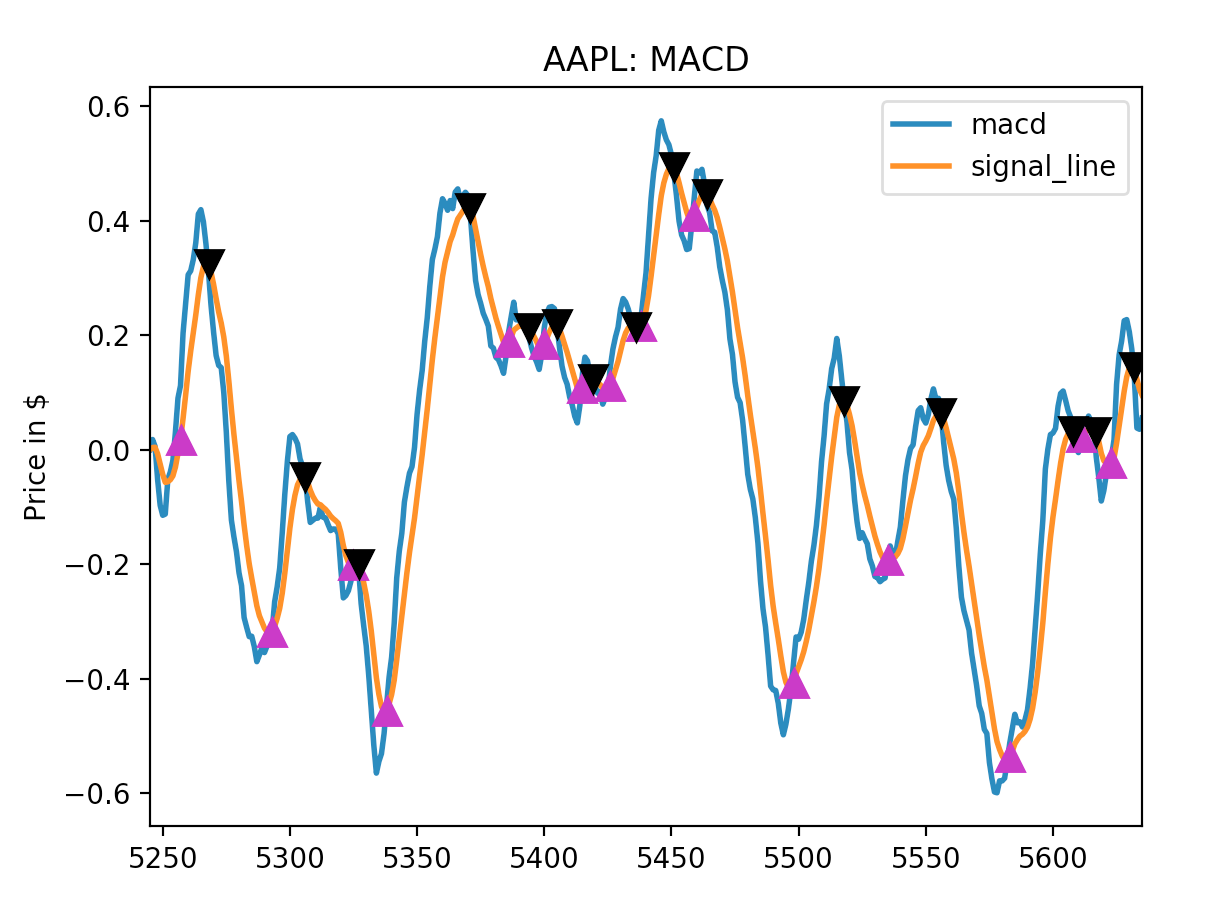
\includegraphics[width=90mm]{AAPL_MACD.png}
\caption{MACD Strategy applied to AAPL \label{overflow}}
\end{figure}

\begin{figure}[ht!]
\centering
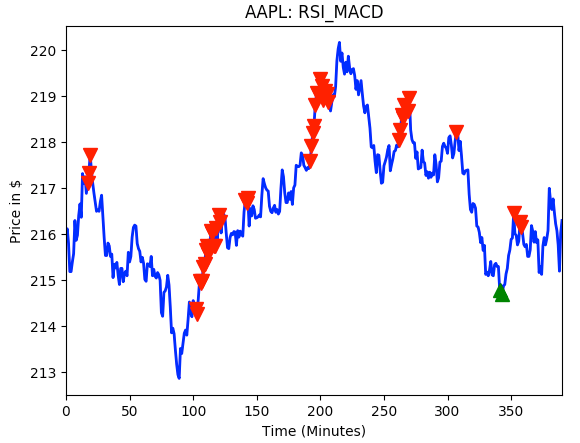
\includegraphics[width=90mm]{AAPL_RSIxMACD.png}
\caption{RSI and MACD strategy buy and sell signals \label{overflow}}
\end{figure}

\section*{Analysis}

\subsection*{Effectiveness}
This strategy takes advantage of using multiple momentum measures to provide more stringent buy signals and less stringent sell signals. This is because both RSI and MACD indicators need to have buy signals whereas only one needs to have a sell signal for a sell off to occur.

\subsection*{Runtime}
The components to consider for this strategy include pulling stock data into a Pandas data frame and calculating rolling means from the data-frame and marking their differences. Pandas is a python data analysis package and is perhaps the most powerful open source data analysis or manipulation tool available. For each calculation, it has to scrape through the entire data-frame at a rolling window, giving a linear runtime.

\subsection*{Quality Metric}
This method is most effective with intraday stock data due to the relative infrequency of buy and sell signals. It was run on 30 stocks on the day of October 26th, 2018 and is compared against a baseline of merely just holding the stock throughout the day. Interestingly, only 11 of the stocks actually generated buy signals for the experiment. However, for each and every stock that had buy signals the strategy  outperformed the baseline, but not by a lot. For example, with the strategy run on AAPL there were .34\% gains while the baseline only having .18\% gains. Another notable result was with VZ with the strategy performing at .01\% and the baseline at -.71\%. This is the first strategy where it would be absolutely necessary to implement this across multiple stocks, as a particular stock can go through multiple days without generating any buy orders. Furthermore, it is worth investigating less stringent buy signals. Rather than having buy orders only come from when both signals match, perhaps having the strategy examine the last 3 minutes to see if both strategies generated buy signals.


\subsection*{Space / Memory Implications}
The only space for RSI and MACD strategy required is the data-frame, which is very reasonable.

\section*{Conclusion}
RSI combined with MACD proves to be a very effective strategy using intraday stock data. Because bullish signals are generated only when both RSI and MACD indicators provide both buy signals, they are far stronger and can be used to purchase larger quantities of stocks at a given time. Also because of this intraday stock usage, this strategy could be implemented to actually trade in real time via Robinhood or a different free-transaction brokerage.

\section*{Implementation}
\begin{verbatim}
def execute(stock, start_date, end_date):
    stock = stockDataRetrieverIntraday(stock, start_date, end_date).getStock()
	
    # create df for both RSI and MACD and merge
    rsi_df = RSI(name, stock)
    macd_df = MACD(name, stock)
    df = pd.merge(rsi_df, macd_df)
    
    # buy signals when both rsi and macd indicate buy
    # sell signals when either one of rsi or macd indicate sell
    df['buy'] = (df['signal_rsi'] == 1) & (df['signal_macd'] == 1)
    df['sell'] = (df['signal_rsi'] == -1) | (df['signal_macd'] == -1)
    df['signal] = df['buy'] + df['sell']

\end{verbatim}

\bibliographystyle{plain}
\bibliography{References}

\end{document}